\documentclass[11pt,twoside]{eitExjobb}
%%\documentclass[11pt,twoside,final]{eitExjobb}  % Use final for the final version that will be printed
%%%%%%%%%%%%%%%%%%%%%%%%%%%%%%%%%%%%%%%%%%%%%%%%%%%%
%% Other fonts (Palatino as rm font, helvetica as sf font and courier as tt font. All fonts are normally installed with a standard LaTeX distribution.)
% \usepackage{mathpazo} % Also in math mode
% \usepackage[scaled=.95]{helvet}
% \usepackage{courier}
%%%%%%%%%%%%%%%%%%%%%%%%%%%%%
% ÅÄÖ
\usepackage[utf8]{inputenc}  % Input encoding (this file): 8 bit unicode. Default by most text editors
\usepackage[T1]{fontenc}     % Output encoding (pdf file)
%%%%%%%%%%%%%%%%%%%%%%%%%%%%%
%% Packages used in the example
\usepackage{graphicx}   % Included graphics and some resizable boxes
\usepackage{url}        % nice urls with line breaks
\usepackage{lipsum}     % nonsense text blocks
%%%%%%%%%%%%%%%%%%%%%%%%%%%%%%
%%%%%%%%%%%%%%%%%%%%%%%%%%%%%%
%%%%%%%%%%%%%%%%%%%%%%%%%%%%%%
\begin{document}
%%% Title page
\Title{Analysis of Analytic Wi-Fi Performance Models Based on End-User Data}
\Author{Axel Smeets\\\texttt{dat12asm@student.lu.se}}
\Supervisor{Björn Landfeld}
\Examiner{Christian Nyberg}
%% Set by default
% \Date{\today}    %% Today's date
% \Year{\the\year} %% This year shown in copyright
% \Company{Department of Electrical and Information Technology\\Lund University}
%%%%%%
\MakeTitlePage  %%% Print title page and copyright page
%%%%%%
\frontmatter    %%% Page numbering for front pages (small roman)

\chapter*{Abstract}
%!TEX root = report.tex

\chapter*{Abstract}

The performance characteristics of Wi-Fi networks have traditionally been
studied and analysed using analytical models and simulations. Due to the
complexity of wireless communication the existing analytical Wi-Fi network
models rely on certain network constraints and simplifications in order to be
mathematically tractable.

We set out to evaluate the practicality of using Wi-Fi performance models to 
estimate network performance by collecting the necessary parameters directly
from an access point. By extension, we must also collect network metrics,
such as packet payload size and number of nodes, for comparison with the model. We 
explore different venues to collect these parameters and metrics to find out
if it is practical to apply the models in Wi-Fi networks. 

After performing three attempts, we conclude that this is difficult due to
several aspects in the Linux kernel, such as batching optimization patterns,
proprietary kernel modules and firmware blobs.


\chapter*{Popular Science Summary}
%!TEX root = base.tex

\chapter*{Popular Science Summary}

% Trådlös kommunikation har växt explosionsartat de senaste årtionden och
% konsumenters krav och förväntningar på bandbredd ökar allt mer. I många hem
% finns trådlösa accesspunkter med stöd för Wi-Fi. De kommer i många skepnader
% - inbakade i en router, som komplement vid sidan av eller i form av s.k.
% "Repeaters".

% Majoriteten av accesspunkter och apparater implementerar Wi-Fi b/g/n vilka kommunicerar via
% radio över frekvensband vid 2.4 GHz. Många modernare accesspunkter lägger även
% till stöd för Wi-Fi ac med frekvensband vid 5 GHz.

% Radiovågors räckvidd är direkt beroende på våglängden och skillnaden i räckvidd
% mellan 2.4 GHz och 5 GHz vara mycket stor. Detta medför att accesspunkter i
% ett hus kan nå in i grannhuset eller lägenheterna runt omkring, och därmed störa
% den trådlösa kommunikationen där, och vice versa.

% För att minimera effekten av denna interferens utnyttjar inte varje accesspunkt
% hela frekvensbandet som standarden tillåter. Istället ska accesspunkterna
% konfigureras så att närliggande accesspunkter inte använder samma del av
% frekvensbandet.

% Det inte finns någon central myndighet, samordning bland tjänsteleverantörer
% eller grannar emellan som genomför denna konfiguration och det är alltså upp
% till den enskilde.

% En stor del av hur en användare upplever nätverket kan därför direkt påverkas av
% hur deras accesspunkt är konfigurerad. Är det många grannar som pratar på samma
% kanaler leder detta till nedsatt prestanda, vilket kan visa sig på många olika
% sätt.

% När kunden inte är nöjd ringer de tjänsteleverantörens support och försöker få
% hjälp. Detta kostar företagen miljonbelopp varje år och oftast måste en tekniker
% skickas ut för att försöka lösa problemet, som egentligen inte ligger på
% leverantörens del av nätet.

% Denna studie har använd data från Telenor med existerande modeller av Wi-Fi-nät
% för att undersöka deras uppförande och se om de överhuvudtaget går att använda.

% Studien har även tagit ett steg till och undersökt om och hur dessa modeller kan
% användas för att estimera Wi-Fi-nätets prestanda vid vissa typer av
% förändringar, t.ex. antalet grannstationer.


%% ToC etc
\tableofcontents
\listoffigures
\listoftables
\cleardoublepage
%%%%% Page numbering for the main thesis (arabic)
\mainmatter
%%%%%

\chapter{Introduction}
\chapter{Introduction}

In 2014 a report on Wi-Fi adoption found that 25\% of households, all over the
world, had Wi-Fi networks set up. In households with fixed-line broadband
access, 65\% had set up a Wi-Fi network\cite{smith}. The report also states that
the number of Wi-Fi-enabled devices is projected to increase.

Naturally, consumers today have higher expectations regarding network throughput
and latency than the IEEE 802.11 standard was designed for back in 1997. In
recent years, the Wi-Fi label has become hugely popular and the standard been
catching up ever since it was introduced beyond the corporate sector, for which
it was originally intended, with almost annual extensions.

One limitation all wireless networking technologies have to consider is radio
interference. Some protocols implement ALOHA-style protocols with no
coordination between devices, relying on collision detection techniques and
subsequent retransmission. IEEE 802.11 implements a \emph{distributed
contribution function} (DCF) which is resposible for controlling access to the
medium.

Even though newer routers today are able to automatically (re)configure
themselves based on analysis of neighbouring networks, they are not guaranteed
to be optimal since they have a local view of the network. Older routers rely on
manual configuration. This configuration is not strictly an issue with the
standard, but rather with how the routers are being deployed. One can think of
the deployment process as being decentralised—each household purchases and
configures their own router.

With existing IEEE 802.11 models it is possible to predict configuration
effects. However, few, if not none, implementations conform to the theoretical
models. This work aims to evaluate IEEE 802.11 models with end-user data and
analyse if, and how, these models may be applicable.

% Centralised configuration is still not on the map for the foreseeable future. Expert systems are already in-place. The task becomes on how to improve existing systems---can we come up with a system which guarantees that a recommended change results in an improvement? This would require extensive simulation of the network and the ability to predict the effect of a change in a configuration parameter.




This master thesis aims to be a step in this direction: evaluate existing Wi-Fi models to see if they are useful in real-world settings.
% em —


% Recommend configuration based on both detailed and wide view of network performance.

% To recommend a change it must lead to improvement in some aspect.

% How to be sure of this? Model the network and simulate what happens when the change is made.

% This requires competent Wi-Fi models.

% Must have clear definition of a competent Wi-Fi model is.

% Wi-Fi models with good performance in simulated tests need not be as good in the real world.

% So we have to test this, and we need the data to do it.

% Telenor now has a good platform for us to get the data.

% But can we trust it? Perhaps the logging is inaccurate?

% So we need to analyse the quality of the data.

%  - is it accurate?
%  - is it precise?

% Experiments will be conducted and results will impact model testing and evaluation.


\chapter{Background}
\chapter{Background}

This chapter provides an overview of the related topics for this master thesis.

\section{TG799-vac}

The OpenWrt-based router examined in this thesis, see Figure \ref{fig:tg799}, is commonly known as TG799, manufactured by Technicolor with Broadcom and Quantenna modems. A custom firmware was used to gain root access over SSH.

\begin{figure}
\center
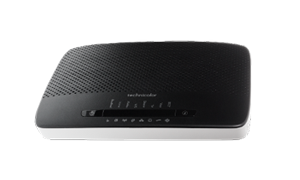
\includegraphics[width=0.5\textwidth]{images/tg799.png}
\caption{The TG799 router from Technicolor}
\label{fig:tg799}
\end{figure}

\section{IEEE 802.11}

The ubiquitous set of LAN standards for wireless communication. Specify MAC and PHY protocols.

Basic protocol description, relevant for this master thesis.

How later standards IEEE 802.11b g n ac change.

\section{ubus - the OpenWrt micro bus architecture}

A client program which acts as an interface to the bus daemon, \texttt{ubusd}. Input and output format is JSON.

The router registers a namespace called \texttt{wireless} and this is what we call to find the meaning of life.

\section{Deutche telekom supra}

Björns oklara vapen.

\section{Rhode \& Schwarz FWLZ-XYZ}

(not broken) network analyser;

\section{Wi-Spy Channalyzer}

the wi-spy, top secret agent auf d00m.

\section{Wireshark}

Wireshark is a well-known program for capturing and inspecting network data.


\chapter{Previous Work}
%!TEX root = base.tex

\chapter{Previous Work}

Modelling of Wi-Fi performance has been an active field of research and this
chapter provides an introduction to the modeling approach described by Bianchi
\cite{bianchi} and subsequent efforts to improve it made by others. In
particular, the studied model presented by Ekici \& Felemban \cite{felemban}
will be discussed.

As mentioned previously, the IEEE 802.11 family specifies the PHY and MAC
layers of WLANs. Analysing the performance impact of these protocols, and 
their numerous parameters, is key to improving network performance. There are
two possible paradigms available: measuring/sampling or constructing an
analytic model of the system/property. Measuring can be done directly on both
physical hardware and software simulations whereas analytical models provide
performance figures as solutions of equations.

The complete behavior of the IEEE 802.11 standards have yet to be captured by
any single analytic model, and researchers instead take the standard
scientific approach of solving a constrained variant of the problem, which in
turn requires rigorous validation of the solution. A model may perform well in
certain conditions and pathologically in others. These behavioural
pecularities arrise from simplification of system behaviour and properties. In
a given model, simplifications can also be inherent in the original
construction mechanism—the way the model itself was constructed—which forces
the model itself to undergo a sort of ironic self-analysis and validation.
Model authors typically present a validation effort to prove their model's
credibility, which further requires scrutiny of the validation itself,
possibly in absurdum...

In short, model authors try to describe a complex system by modelling key
components in a constrained setting, and validate their model using other
models which have been more thoroughly reviewed. 

Given this context, we first present the original Markov-Chain model from
\cite{bianchi} and describe how it models IEEE 802.11 properties using the
DCF, some significant and intentional simplifications made and a narrow
selection of subsequent contributions made by others $refs$. % TODO: ADD REFS

Finally, the evaluated model \cite{felemban} is described as well as the
differences to both the original model \cite{bianchi} and some intrinsic model
properties useful in forthcoming chapters.

\section{The Bianchi Model}

In \cite{bianchi}, Bianchi presented a novel approach to modeling IEEE 802.11
performance by creating a Markov chain model of the \emph{Distributed
Coordination Function} (DCF). Bianchi defines three important properties:
transmission probability, normalised throughput and channel access delay. This
section provides a summary of the original model and definitions useful in
later chapters.

Before going into detail about the Bianchi model, we start from the beginning.

The underlying assumption of a MAC-layer-based model of IEEE 802.11 is that,
in a setting with more than 2 STAs, the MAC protocol should be the system
bottleneck. By extension, it is reasonable to model the performance of the
network based on the DCF. 

In \cite{bianchi}, Bianchi starts by limiting the proposed model analysis to
fully-connected, single-hop networks in ``saturation''. The saturation
condition requires that all STAs, at any point in time, always want to
transmit. This allows Bianchi to omit send queue distributions and simplify
collision probabilities, which will become important. Additionally, Bianchi
assumes that there is a fixed number of $N$ equivalent, contending STAs.

The back-off counter for a given STA at time $t$ is represented by the
stochastic process $b(t)$. Since the back-off counter at any given time $t$ is
dependent on the transmission history it follows that $b(t)$ is non-Markovian.
To solve this problem Bianchi assumes that each transmission attempt collides
with a constant and independent probability $p$.

In addition to the back-off counter process, $b(t)$, Bianchi also introduces a
stochastic process $s(t)$ representing the current back-off stage for a given
STA at time $t$. Recall from Equation \ref{eq:mlog} that $m$ is the number of
back-off stages, from which the states of $s(t)$ can be obtained as $(0,
\dots, m)$.

After breaking the historical dependency of the back-off process, Bianchi can
model the time-discrete bidimensional process $\{s(t), b(t)\}$ as the Markov
chain seen in Figure \ref{fig:tnmc}. As seen in the figure, the model ignores
several important behaviors of the DCF, in particular retransmission limit and
backoff counter freezing due to channel state.

\begin{enumerate}

	\item \textbf{Retransmission Limit} - the model does not drop the packet
after failing \texttt{ShortRetryLimit} retransmissions, instead it continues
until the packet has been successfuly acknowledged.

	\item \textbf{Back-off Counter Freezing} - in each back-off state, the
probability of decrementing the back-off counter—equivalent to sensing the
channel idle—is always 1.

\end{enumerate}

Bianchi assumes that the conditional collision probability $p$ is constant and
independent of the back-off stage. This implies that $p$, the probability of
an STA encountering collision during transmission, is equivalent to the
probability that any of the other $N-1$ STAs also attempted to transmit, with
transmission probability $\tau$

\begin{equation} \label{eq:pbi}
	p = 1 - (1 - \tau)^{N-1}
\end{equation}

By modelling the back-off counter itself, combined with the saturation
condition and omission of retransmission limit, Bianchi solves the
transmission probability $\tau$ by essentially finding the steady state
probability of the back-off counter being zero, and obtains

\begin{equation} \label{eq:xbi}
	\tau = \frac{2(1-2p)}{(1-2p)(\mathit{CW_{min}}+1)+p\mathit{CW_{min}}(1-(2p)^m)}
\end{equation}

However, since $\tau$ is derived from the back-off counter, and the back-off
counter depends on the conditional collision probability $p$, it follows that
$\tau$ and $p$ are recursively defined. Bianchi constructs a nonlinear system
with equations for $\tau$ and $p$ and solves it numerically.

With probabilities for $\tau$ and $p$, Bianchi continues to his core
contribution—the normalised throughput. Denoted $S$, it is defined as ``the
fraction of time the channel is used to transmit payload bits''. 

\begin{equation} \label{eq:ssbi}
	S = \frac{E[\mathit{payload~information~transmitted~in~a~slot~time}]}{E[\mathit{length~of~slot~time}]}
\end{equation}

With $E[P]$ denoting mean payload size, probabilities for transmission
$P_{tr}$ and transmission success $P_S$, the numerator in \ref{eq:ssbi}
becomes $P_S P_{tr} E[P]$. In a similar fashion, the denominator in
\ref{eq:ssbi} can be expressed as the sum of empty time slots, busy time slots
and times slots with collisions. Let $\sigma$ be the duration of an empty
slot, $T_{S}$ the average time the channel is sensed busy in case of
successful transmission, and $T_{C}$ the average time the channel is sensed
busy in case of collision for the non-colliding STAs. Now, Bianchi presents an
equation for the normalized througput $S$

\begin{equation} \label{eq:sbi}
	S = \frac{P_S P_{tr} E[P]}{(1-P_{tr})\sigma + P_{tr} P_S T_S + P_{tr} (1-P_S) T_C}
\end{equation}

Note that $S$ is expressed independent from the ``access modes'' found in
Figure \ref{fig:timings}, which details the communication flow of a single,
successful packet transmission and acknowledgement. Let $H = T_{\mathit{PHY}}
+ T_{\mathit{MAC}}$ and assume propagation delay $\delta$. The differences
between the ``access modes'' can thus captured by the variables $T_{S}$ and
$T_{C}$

\begin{align}  \label{eq:tbi}
	\mathit{basic} & \left\{
		\begin{aligned}
	        T^{bas}_{S} & = H + E[P] + \mathit{SIFS} + \delta + \mathit{ACK} + \mathit{DIFS} + \delta  \\
	        T^{bas}_{C} & = H + E[P] + \mathit{DIFS} + \delta
	    \end{aligned}
	\right. \\
	\mathit{RTS/CTS} & \left\{
	    \begin{aligned}
	        T^{rts}_{S} = & ~ \mathit{RTS} + \mathit{SIFS} + \delta + \mathit{CTS} + \mathit{SIFS} + \delta \\ & + H + E[P] + \mathit{SIFS} + \delta + \mathit{ACK} + \mathit{DIFS} + \delta  \\
	        T^{rts}_{C} = & ~ \mathit{RTS} + \mathit{DIFS} + \delta
	    \end{aligned}
	\right.
\end{align}


From these equations Bianchi concludes that for any network of size $N$ there
exists a troughput-optimal transmission probability $\tau$, achievable by
tuning the congestion window sizes and $\mathit{CW_{min}}$ and $\mathit{CW_{max}}$.

To make the model tractable Bianchi simplifies many behaviours, of which two
have received considerable efforts to implement. Some notable publications 
are Wu \cite{1019305} and Chatzimisios \cite{1258379}, who proposed improved
models that included the retransmission limit, followed by Zhang
\cite{article} and Xiao \cite{1512111}, who proposed models that include
back-off counter freezing.

\begin{figure}
\center
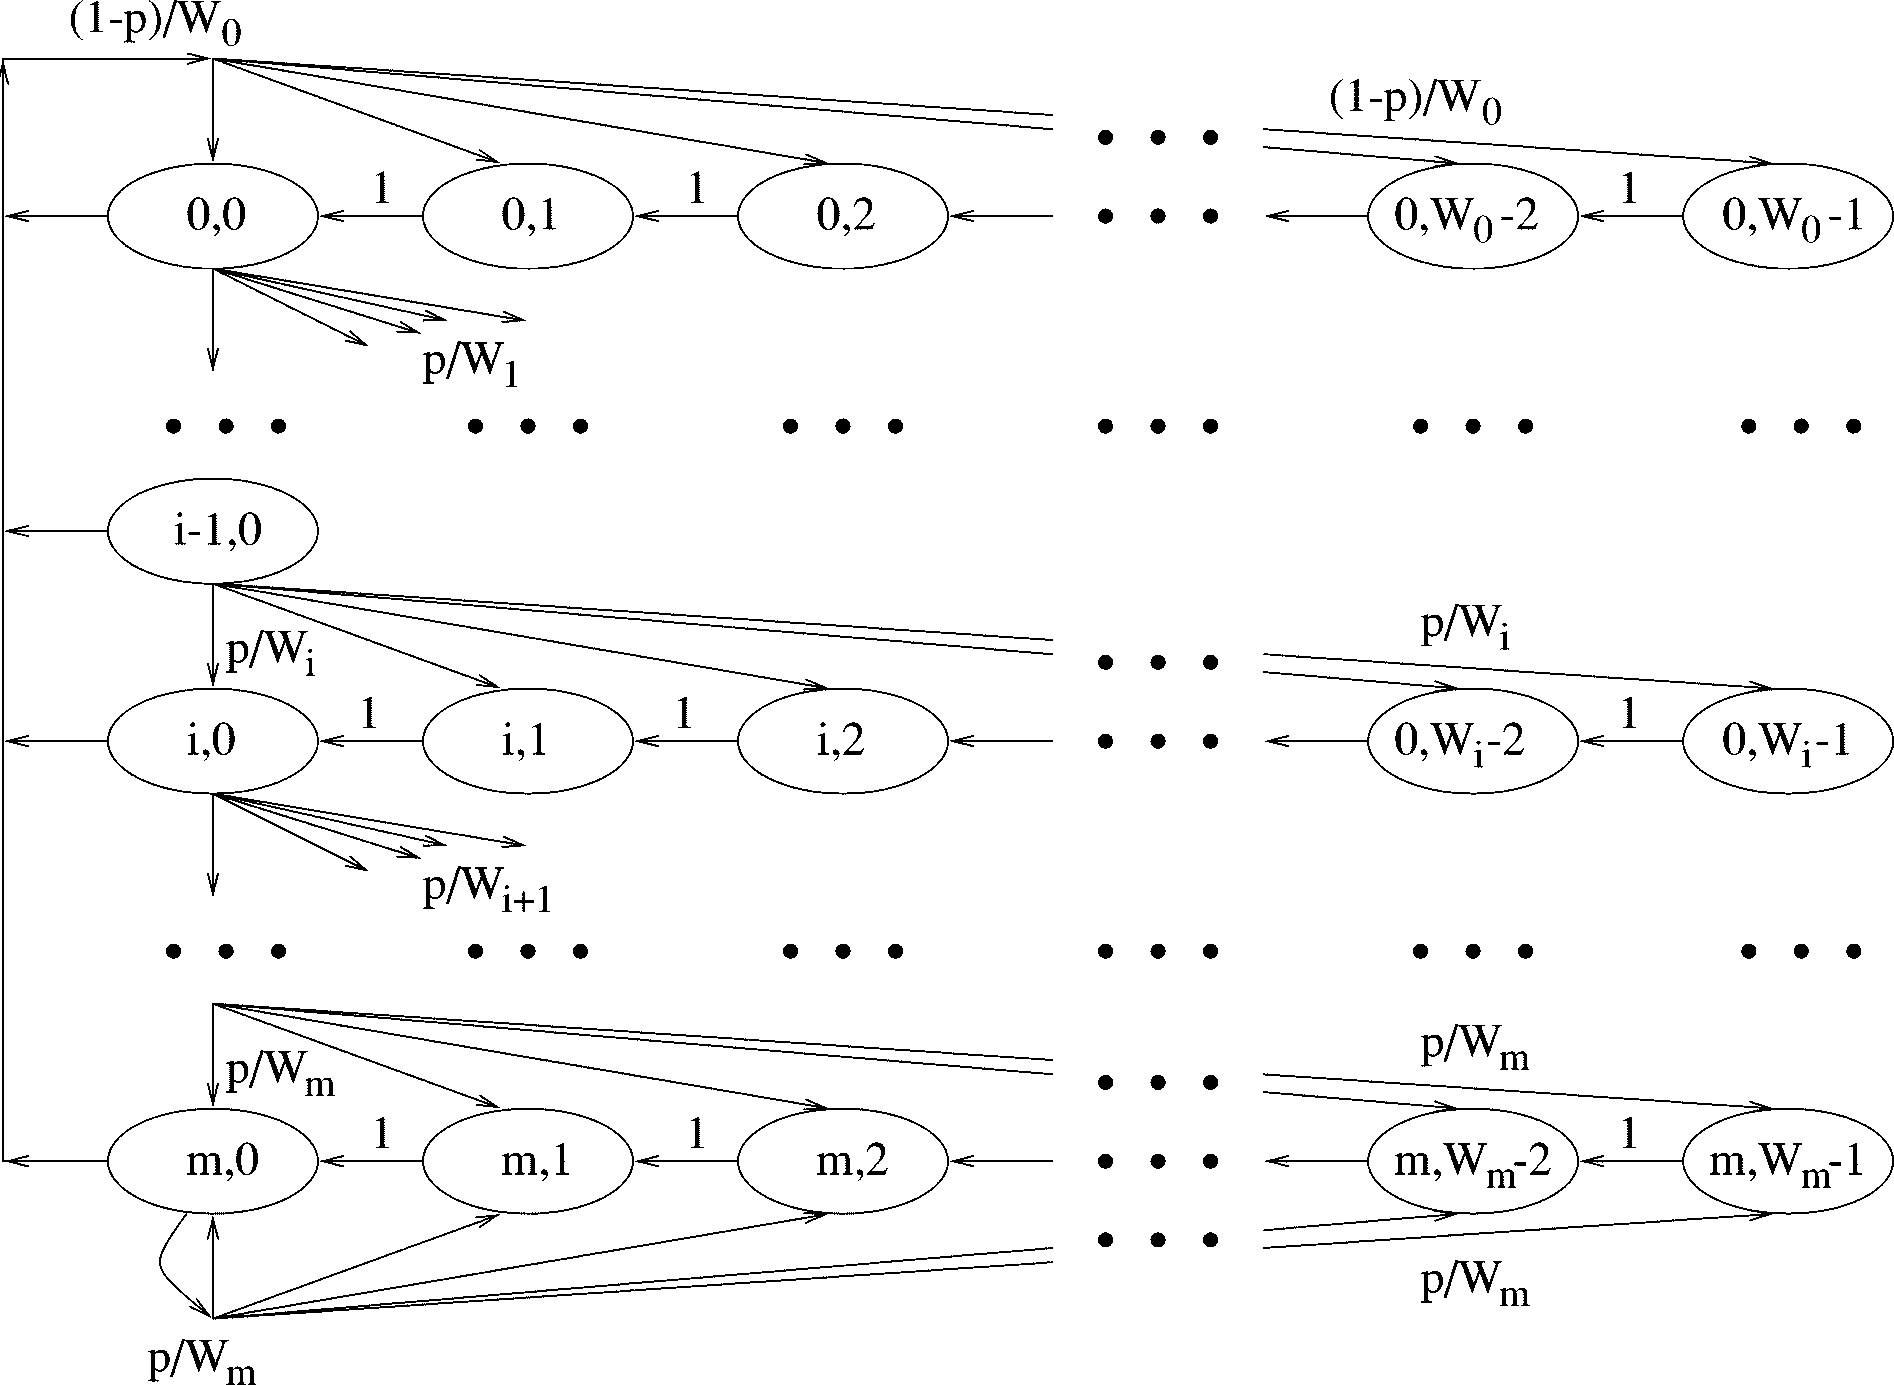
\includegraphics[width=0.9\textwidth]{images/bianchi-model.png}
\caption{Bianchi's \emph{Tagged-Node Markov Chain} model of the IEEE 802.11 DCF where $p$ is the collision probability, $W_i$ the contention window size at attempt $i$ ($0 \leq i \leq m$) and $m$ from Equation \ref{eq:mlog}.}
\label{fig:btnmc}
\end{figure}

\section{The Felemban-Ekici Model}

A decade later, in 2011 specifically, Felemban \& Ekici published an extended
version of Bianchi's model, where they significantly improved the model's
accuracy by introducing a more accurate behaviour of the entry into backoff
and the backoff countdown procedures \cite{felemban}.

An overview of the TNMC model from \cite{felemban} is presented in Figure
\ref{fig:tnmc}. Some differences compared to Bianchi's TNMC are inclusion of
retransmission limit (in state $\{0,L\}$, collision results in packet drop)
and counter freezing $P_f$ (probability of state a $\{i,j\}$ transitioning to itself).

The inclusion of retransmission limits results in a different expression of
$\tau$ compared to Equation \ref{eq:xbi}. Recall from Equation \ref{eq:cwj}
that $W_j$ is the size of the contention window at back-off stage $j$ and that
$L$ is the short retry limit from \cite{654749}. Felemban \& Ekici solves
$\tau$ similarly to \cite{bianchi} by finding the probability of the back-off
counter reaching 0 in all back-off stages, expressed as

\begin{equation} \label{eq:xfe}
	\tau = \frac{1-P^{L+1}}{
		(\Sigma^L_{j=0}
			[1 + \frac{1}{1-P_f}
				\Sigma^{W_j-1}_{k=1} \frac{W_j-k}{W_j}
			]
		)(1-P)}
\end{equation}

where $P$ is the conditional collision probability (equivalent to $p$) from
Equation \ref{eq:pbi}.

\begin{align}  \label{eq:tfe}
	\mathit{basic} & \left\{
	        T^{bas}_{C} = T^{bas}_{S} = \mathit{DIFS} + T_h + T_p + \mathit{SIFS} + \mathit{ACK}
	\right. \\
	\mathit{RTS/CTS} & \left\{
	    \begin{aligned}
	        T^{rts}_{S} = & ~ \mathit{DIFS} + T_\mathit{RTS} + \mathit{SIFS} + T_\mathit{CTS} \\ & + \mathit{SIFS} + T_h + T_p + \mathit{SIFS} + \mathit{ACK}  \\
	        T^{rts}_{C} = & ~ \mathit{DIFS} + T_\mathit{RTS} + \mathit{SIFS} + T_\mathit{CTS}
	    \end{aligned}
	\right.
\end{align}

As shown in Figure \ref{fig:dcfgraph}, the DCF back-off process algorithm
specifies that a node only decrements the back-off counter if the channel was
sensed idle. In \cite{felemban}, the authors obtained an accurate countdown
probability ($P_d$) by introducing an additional markov chain to model the
channel-sensing process and estimating the probability of \emph{not} counting
down, i.e. probability of counter freeze ($P_f$). This chain is called
Channel-Sense Markov Chain (CSMC). The counter freeze probability, $P_f$, is
computed by finding the steady state probabilities of the CSMC by fixed point
iteration.

The addition of CSMC and $P_f$ increased the model's accuracy significantly
compared to other models in various test conditions. In particular, the
introduction of $P_f$ increased accuracy of the model when extended to
\emph{unsaturated} networks.

While the model proposed by Ekici-Felemban models the DCF more closely and
accurately, several assumptions and omissions, in addition to constraints
inherited from the markov chain approximation, makes the model a very
interesting candidate for real-world testing. 

\begin{figure}
\center
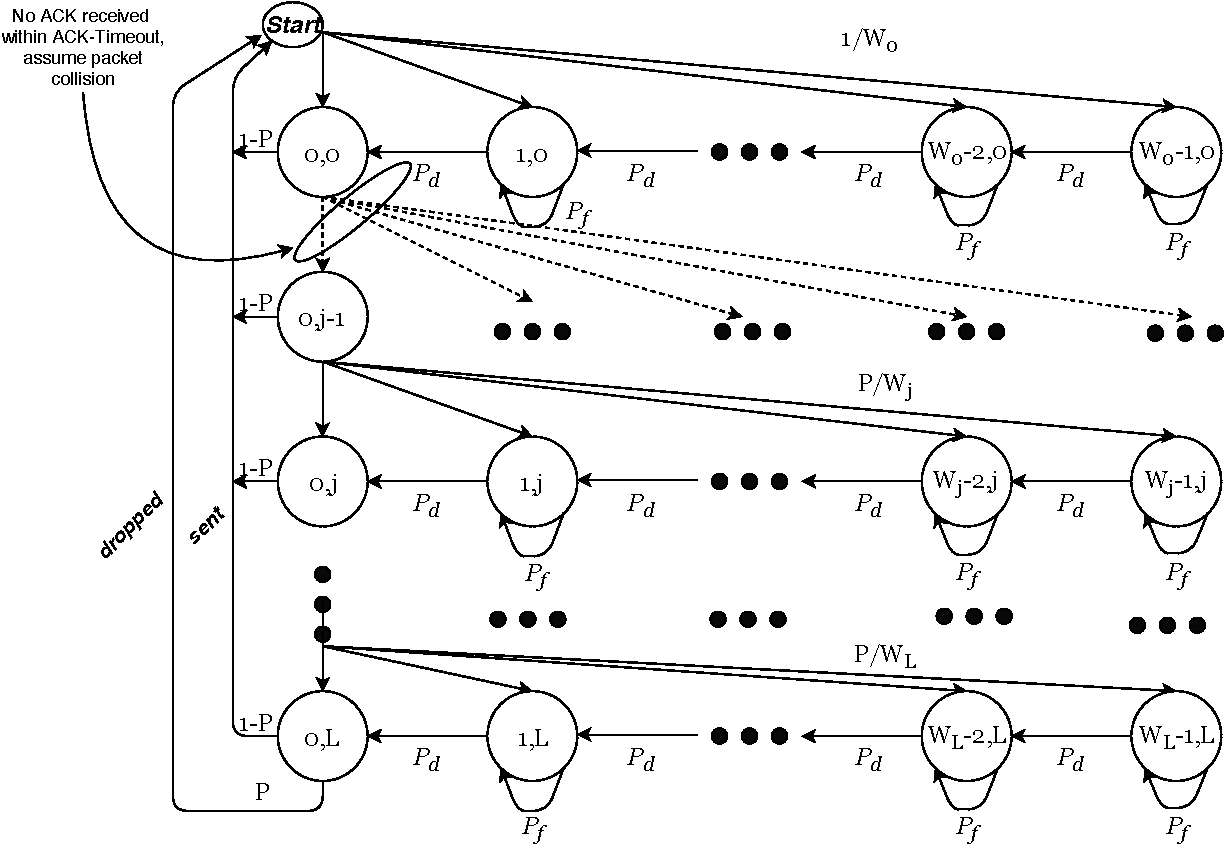
\includegraphics[width=1\textwidth]{images/tnmc-dcf.pdf}
\caption{Ekici-Felemban's Tagged-Node Markov Chain (TNMC) model of the IEEE 802.11 DCF. $P$ is packet collision probability, $P_d$ is probability to decrease backoff counter, $P_f = 1 - P_d$, $W_j$ is contention window size at attempt $j$ and $L$ is the Short Retry Limit}
\label{fig:tnmc}
\end{figure}

\subsection{The Unsaturated Model}

Recall that the original Bianchi model assumed that the network was in
\emph{saturation} conditions, i.e. all STAs always have something in their
send buffer. After presenting the improved model in \cite{felemban}, 
extended to work in \emph{unsaturated} networks.

\chapter{Results}
In Figure~\ref{fig:testfig} a typical test mage is shown.
\begin{figure}[htbp]
  \centering
  \includegraphics[width=0.4\linewidth]{example-image}
  \caption{Example image.}
  \label{fig:testfig}
\end{figure}

\section{New new section}
\lipsum[1-2]
\begin{table}[htbp]
  \centering
  \begin{tabular}{lll}
    Group & Test 1 & Test 2\\\hline
    A & 253 &54\\
    B & 636 & 33
  \end{tabular}
  \caption{A nice table.}
  \label{tab:tabletest}
\end{table}

\lipsum[3]
\begin{figure}[htbp]
  \begin{minipage}[t]{0.5\linewidth}
    \centering
    \includegraphics[width=0.8\linewidth]{example-image-a}
    \caption{Image A}
    \label{fig:imageA}
  \end{minipage}%
  \begin{minipage}[t]{0.5\linewidth}
    \centering
    \includegraphics[width=0.8\linewidth]{example-image-b}
    \caption{Image B. It can also be a long caption even if the space is narrow.}
    \label{fig:imageB}
  \end{minipage}
\end{figure}

Figure~\ref{fig:imageA} is displayed next to Figure~\ref{fig:imageB}. Notice that \verb|\linewidth| is the line width inside the \verb|minipage|.

\lipsum[4]


\chapter{Discussion and Future Work}
If you want to know more about \LaTeX\ there is a (free) manual at \cite{cite:NotShort}. For more specific questions, it is recommended to have a look at the forum StackExchange \cite{cite:TeX.SX}, where the most common questions already have answers. All official packets can be found, and downloaded, from CTAN \cite{cite:CTAN}. Finally, for the hardcore programmer who thinks \LaTeX\ is a bit inflexible, I can recommend the \TeX\ introduction in \cite{cite:TeXimpatient}.

For questions about how you should do to get your imported graphics as you want, have a look at \cite{cite:ImportedGraphics}. If you instead want to do the images inline from the \TeX\ code you are recommended to use TikZ \cite{cite:TikZ}. However, it is known to have a relatively high learning threshold.


%%%%%%%%%%%%%%%%%%%%%%%%%%%%%%%%%%%%%%%
%% References
\begin{thebibliography}{99}
\bibitem{cite:NotShort} T. Oetiker, H Partl, I Hyna, and E. Schlegl, \textit{A (Not So) Short Introduction to \LaTeX2e}, \url{www.ctan.org/tex-archive/info/lshort/english/}
\bibitem{cite:TeX.SX} \{\TeX\} StackExchange, \url{tex.stackexchange.com/}
\bibitem{cite:CTAN} The Comprehensive \TeX\ Archive Network, \url{www.ctan.org/}
\bibitem{cite:TeXimpatient} P. Abrahams, K. Hargreaves, and K. Berry, \textit{TeX for the Impatient}, \url{savannah.gnu.org/projects/teximpatient/}
\bibitem{cite:ImportedGraphics} K. Reckdahl, \textit{Using Imported Graphics in LaTeX and pdfLaTeX}, \url{www.ctan.org/tex-archive/info/epslatex/english}
\bibitem{cite:TikZ} T. Tantau, \textit{The TikZ and PGF Packages}, \url{www.bu.edu/math/files/2013/08/tikzpgfmanual.pdf}. Warning: 400+ pages.
\end{thebibliography}


%%%%%%%%%%%%%%%%%%
\appendix
%%%%%%%%%%%%%%%%%%
\chapter{Some extra material}
\lipsum[1]
\begin{figure}[htbp]
  \centering
  \includegraphics[width=0.6\linewidth]{example-image}
  \caption{A picture or table in the appendix is numbered accordingly.}
  \label{fig:AppFig}
\end{figure}

\end{document}
